% Copyright (c) 2023 Jesse Straat
% 
% This software is released under the MIT License.
% https://opensource.org/licenses/MIT

\makeatletter
\def\input@path{{../}}
\makeatother
\documentclass{scripts/preamble}

\usepackage{docmute}



% different page numberings
\newcommand\frontmatter{%
    \cleardoublepage
    \pagenumbering{roman}}% Lowercase Roman numbers

\newcommand\mainmatter{%
    \cleardoublepage
    \pagenumbering{arabic}}% Normal numbers

\newcommand\backmatter{%
    \cleardoublepage
    \pagenumbering{Roman}% Capital Roman numbers
    \pagestyle{plain}}


% If you want an index:
% \makeindex[intoc]

% Saving theorems to a file
\theoremfile

\begin{document}
\pagenumbering{alph}% We don't want the title page to be page 1
% Copyright (c) 2023 Jesse Straat
% 
% This software is released under the MIT License.
% https://opensource.org/licenses/MIT

% This title page was inspired by one made by A-Eskwadraat's TeXniCie

%!TeX root = titlepage

\documentclass[12pt]{report}

\makeatletter
\def\input@path{{../}}
\makeatother
\usepackage{scripts/preamble}

\begin{document}
	\newgeometry{margin=1.5cm}
	\begin{titlepage} % Special titlepage environment
		\noindent
		\begin{minipage}{0.4\textwidth}
			
\includegraphics[width=\linewidth]{images/uulogo} % UU logo --- replace with own logo
		\end{minipage}
	
	    \par\vspace{0.3cm}
	    
	    \begin{flushright}
	    {\Large\bfseries Bachelor'r programma\\\LaTeX \par} % Space for faculty/programme
	    \end{flushright}
		\vspace{0.3cm}
	    \begin{center}
	    {\LARGE\bfseries A catchy title:\par} % Title
	    {\Large\bfseries A catchier subtitle\par}
	    \end{center}
		\vspace{1cm}
	    {\scshape\Large Thesis\par}
		\vspace{0.5cm} % Specify the type of thesis: is it for your bachelor's or your master's, or.... 
		{\Large\itshape Jesse Straat\par} % Name
	    \vspace{0.5cm}
	    \centering
	    \fbox{% This adds a black border around your picture
	    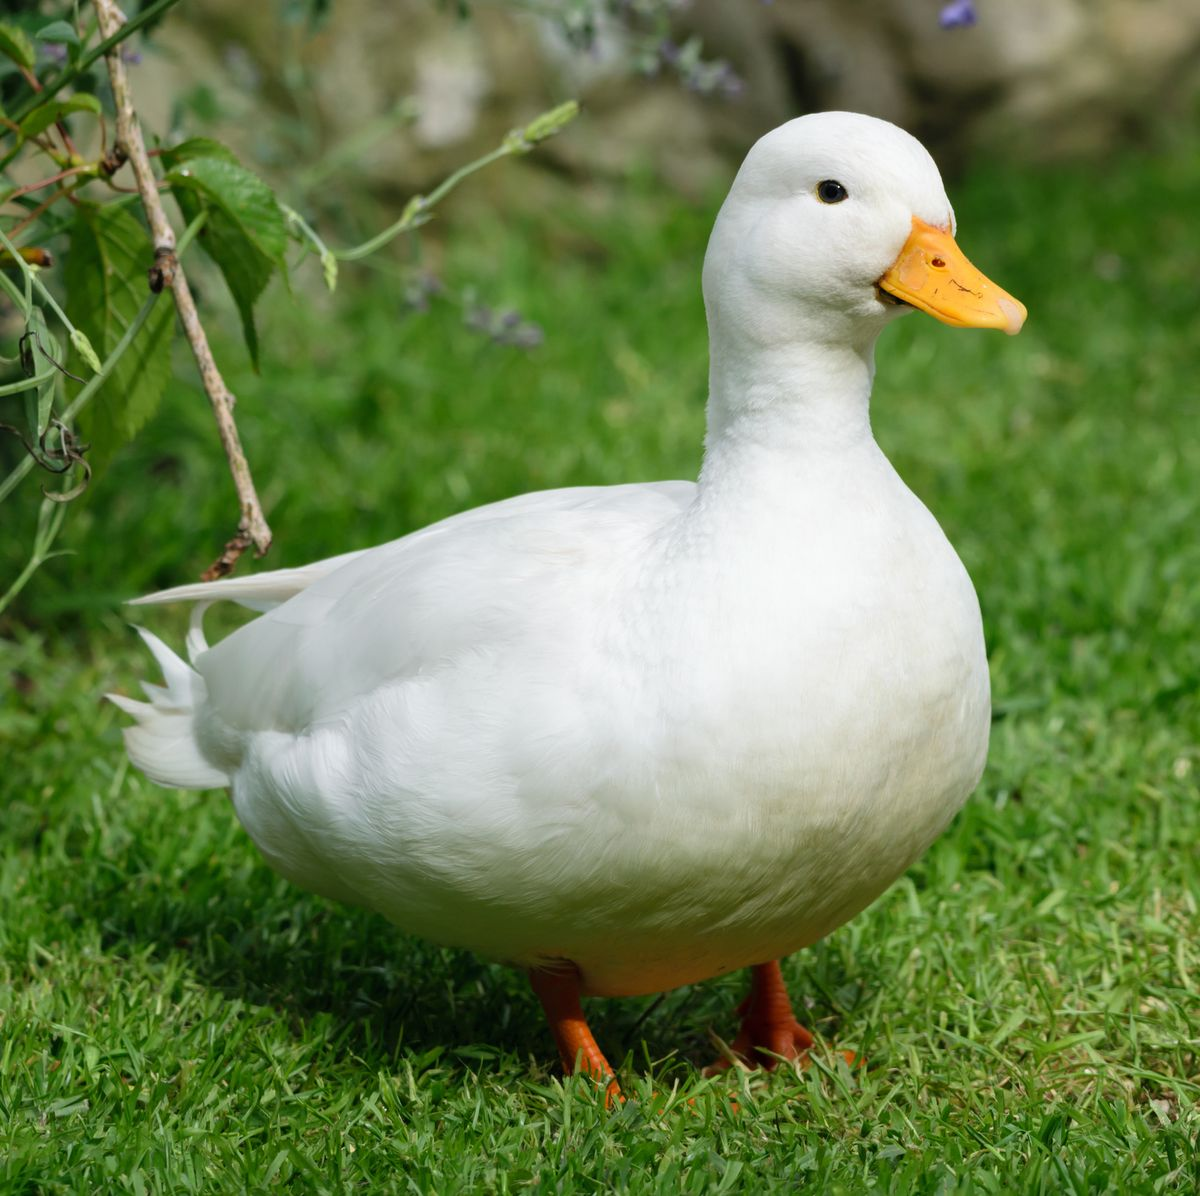
\includegraphics[height=0.3\textheight]{images/duck} % Insert picture here
	    % Adjust height if necessary
	    }%
	    \vspace{0.5cm}
	    \par
	    \raggedleft
		{\Large\itshape Supervisors}:\par\vspace{0.25cm}% Here is some space for your supervisors
		%
        {\large Prof. Dr \textsc{Alice Ashley}\par}% First supervisor
	    Institute for \LaTeX{} templates\par% Institute
	    \vspace{0.25cm}
        %
	    {\large Prof. Dr \textsc{Bob Bobbington}\par}% Second supervisor
	    \TeX nical Institute\par% Institute
	    \vspace{0.25cm}
        % Repeat for additional supervisors
		\vfill
		{\large \today\par}% Replace \today with the date of your choice if needed
	    
	\end{titlepage}    
	%
	\restoregeometry
\end{document}
%
\frontmatter % We want lowercase roman numerals here. 
%
% Copyright (c) 2023 Jesse Straat
% 
% This software is released under the MIT License.
% https://opensource.org/licenses/MIT

%!TeX root = abstract

\makeatletter
\def\input@path{{../}}
\makeatother
\documentclass{scripts/preamble}

\begin{document}
    \newgeometry{margin=2.5cm}
	\begin{abstract}
		\thispagestyle{plain}
		\noindent
		This is an abstract.
	\end{abstract}
	%
	\restoregeometry % Resets geometry
\end{document} % Abstract
%
\clearpage % Contents on next page
\setcounter{tocdepth}{2} % Change integer to desired number of columns in table of contens
\tableofcontents % Generates the table of contents
%
\mainmatter % We want normal pagenumbers from now on
%
% Copyright (c) 2023 Jesse Straat
% 
% This software is released under the MIT License.
% https://opensource.org/licenses/MIT

%!TeX root = introduction

\documentclass[12pt]{article}

\makeatletter
\def\input@path{{../}}
\makeatother
\usepackage{scripts/preamble}

\begin{document}
	\section*{Introduction\markboth{Introduction}{}}
	\addcontentsline{toc}{section}{\protect\numberline{}Introduction}		% Makes sure that the introduction has no number but is in table of contents
	This is an introductory story.
	%
	\clearpage
	%
	\subsection*{Organisation}
	Here's what each chapter is going to be about.
	%
	\subsection*{Preliminaries}
	You should know Category Theory for this thesis\cite{rudin_principles_1976}.
	%
	\subsection*{Notation and conventions}
	Here, I introduce my conventions.
    %
	\subsubsection*{A summary of mathematical notation}
    Here is a table of mathematical notation that will be used in this thesis.\\
	{\renewcommand\tabularxcolumn[1]{m{#1}}
	\renewcommand{\arraystretch}{1.5}
	\begin{tabularx}{\textwidth}{ c X }
		\(\qed\) & This symbol denotes the end of a proof.
	\end{tabularx}}
	%
	\subsection*{Acknowledgements}
	I would like to thank myself for making this template. My cat deserves praise for being cute.
	\makethm{theorem}{thm:stest}{TEST\\TEST\par TEST}
	\repthm{theorem}{thm:stest}
\end{document}
%
% Copyright (c) 2023 Jesse Straat
% 
% This software is released under the MIT License.
% https://opensource.org/licenses/MIT

%!TeX root = chapter1

\documentclass[12pt]{article}

\makeatletter
\def\input@path{{../}}
\makeatother
\usepackage{scripts/preamble}

\begin{document}
    \section{Category Theory}\label{sec:simps}
    A monad is a monoid in the category of endofunctors.
    \makethm{theorem}{thm:sstest}[Yoneda Lemma]{Everything that I claim is true.}
\end{document}
%
% For new chapters, use 
% \clearpage
% \input{subfiles/chapter}
%
\backmatter % Capital romans from here on
%
\DeclareFieldFormat{url}{\linebreak\url{#1}} % Fixes urls in bibliography
\printbibliography[heading=bibintoc]
%
% If you want an index:
% \clearpage
% \printindex
\end{document}

